\section{Referencia de la Estructura enunciado\-For}
\label{structenunciadoFor}\index{enunciadoFor@{enunciadoFor}}
Clase de almacenamiento de enunciados for en el AST.  


{\tt \#include $<$ast.h$>$}

Diagrama de colaboraci\'{o}n para enunciado\-For:\begin{figure}[H]
\begin{center}
\leavevmode
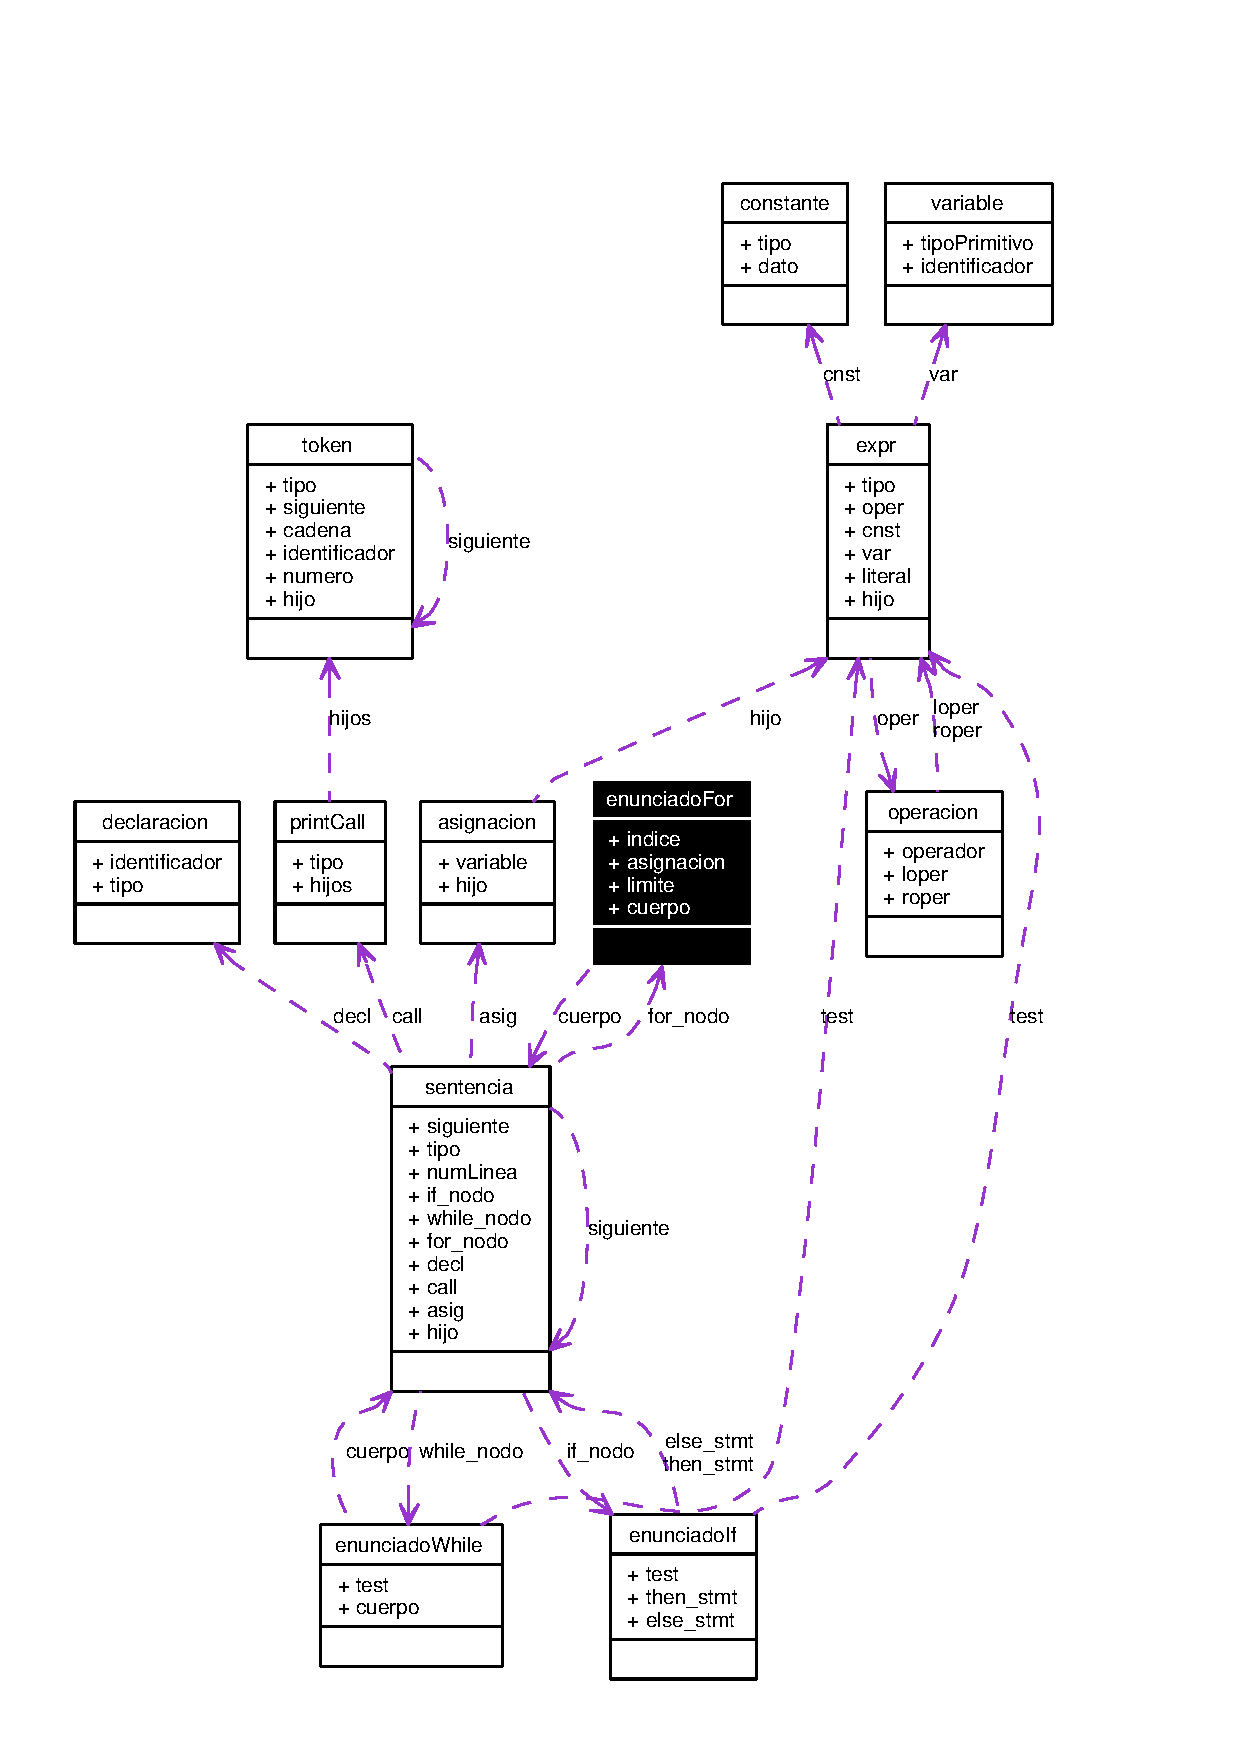
\includegraphics[width=263pt]{structenunciadoFor__coll__graph}
\end{center}
\end{figure}
\subsection*{Atributos p\'{u}blicos}
\begin{CompactItemize}
\item 
char $\ast$ {\bf indice}
\begin{CompactList}\small\item\em Identificador indice que apunta a variable entera. \item\end{CompactList}\item 
int {\bf asignacion}
\begin{CompactList}\small\item\em Entero a asignar a variable. \item\end{CompactList}\item 
int {\bf limite}
\begin{CompactList}\small\item\em Entero limite del ciclo. \item\end{CompactList}\item 
{\bf sentencia} $\ast$ {\bf cuerpo}
\begin{CompactList}\small\item\em Cuerpo de sentencias a evaluar. \item\end{CompactList}\end{CompactItemize}


\subsection{Descripci\'{o}n detallada}
Clase de almacenamiento de enunciados for en el AST. 



Definici\'{o}n en la l\'{\i}nea 197 del archivo ast.h.

\subsection{Documentaci\'{o}n de los datos miembro}
\index{enunciadoFor@{enunciado\-For}!asignacion@{asignacion}}
\index{asignacion@{asignacion}!enunciadoFor@{enunciado\-For}}
\subsubsection{\setlength{\rightskip}{0pt plus 5cm}int {\bf enunciado\-For::asignacion}}\label{structenunciadoFor_o1}


Entero a asignar a variable. 



Definici\'{o}n en la l\'{\i}nea 199 del archivo ast.h.

Referenciado por evaluar\-For(), y insertar\-Ciclo\-For().\index{enunciadoFor@{enunciado\-For}!cuerpo@{cuerpo}}
\index{cuerpo@{cuerpo}!enunciadoFor@{enunciado\-For}}
\subsubsection{\setlength{\rightskip}{0pt plus 5cm}{\bf sentencia}$\ast$ {\bf enunciado\-For::cuerpo}}\label{structenunciadoFor_o3}


Cuerpo de sentencias a evaluar. 



Definici\'{o}n en la l\'{\i}nea 201 del archivo ast.h.

Referenciado por borrar\-For(), evaluar\-For(), y insertar\-Ciclo\-For().\index{enunciadoFor@{enunciado\-For}!indice@{indice}}
\index{indice@{indice}!enunciadoFor@{enunciado\-For}}
\subsubsection{\setlength{\rightskip}{0pt plus 5cm}char$\ast$ {\bf enunciado\-For::indice}}\label{structenunciadoFor_o0}


Identificador indice que apunta a variable entera. 



Definici\'{o}n en la l\'{\i}nea 198 del archivo ast.h.

Referenciado por borrar\-For(), evaluar\-For(), y insertar\-Ciclo\-For().\index{enunciadoFor@{enunciado\-For}!limite@{limite}}
\index{limite@{limite}!enunciadoFor@{enunciado\-For}}
\subsubsection{\setlength{\rightskip}{0pt plus 5cm}int {\bf enunciado\-For::limite}}\label{structenunciadoFor_o2}


Entero limite del ciclo. 



Definici\'{o}n en la l\'{\i}nea 200 del archivo ast.h.

Referenciado por evaluar\-For(), y insertar\-Ciclo\-For().

La documentaci\'{o}n para esta estructura fu\'{e} generada a partir del siguiente archivo:\begin{CompactItemize}
\item 
/media/docs/progra/c++/compiladores1/proy2/godzilla/src/{\bf ast.h}\end{CompactItemize}
